El Nivel Regulatorio constituye el sistema de control en tiempo real del robot, implementado en un microcontrolador Arduino Mega 2560. Su responsabilidad principal es la gestión directa de actuadores (motores paso a paso, servomotores, gripper) y sensores (finales de carrera), ejecutando comandos de movimiento con precisión temporal estricta.

\subsubsection{Estructura del Firmware}

El firmware se organiza en módulos funcionales que implementan el patrón de diseño de capas (Figura \ref{fig:arquitectura_regulatorio}):

\textbf{Capa de Drivers}:
\begin{itemize}
    \item \texttt{stepper\_driver}: Generación de pulsos para motores paso a paso vía Timer1
    \item \texttt{servo\_driver}: Control PWM de servomotores vía Timer4 y Timer5
    \item \texttt{gripper\_driver}: Control del motor paso a paso 28BYJ-48 del gripper
    \item \texttt{uart\_driver}: Comunicación serial con buffer circular interrupt-driven
    \item \texttt{encoder\_driver}: Lectura de encoders incrementales (futuro)
\end{itemize}

\textbf{Capa de Control}:
\begin{itemize}
    \item \texttt{motion\_profile\_simple}: Generación de perfiles trapezoidales de velocidad
    \item \texttt{limits}: Gestión de finales de carrera y detención por límites
    \item \texttt{moves}: Coordinación de movimientos multi-eje
\end{itemize}

\textbf{Capa de Aplicación}:
\begin{itemize}
    \item \texttt{command\_parser}: Interpretación de comandos UART
    \item \texttt{command\_protocol}: Definición del protocolo de comunicación
    \item \texttt{system\_config}: Parámetros de configuración centralizados
\end{itemize}

\begin{figure}[H]
    \centering
    % TODO: Insertar diagrama de capas del firmware regulatorio
    % Mostrar: Aplicación → Control → Drivers → Hardware
    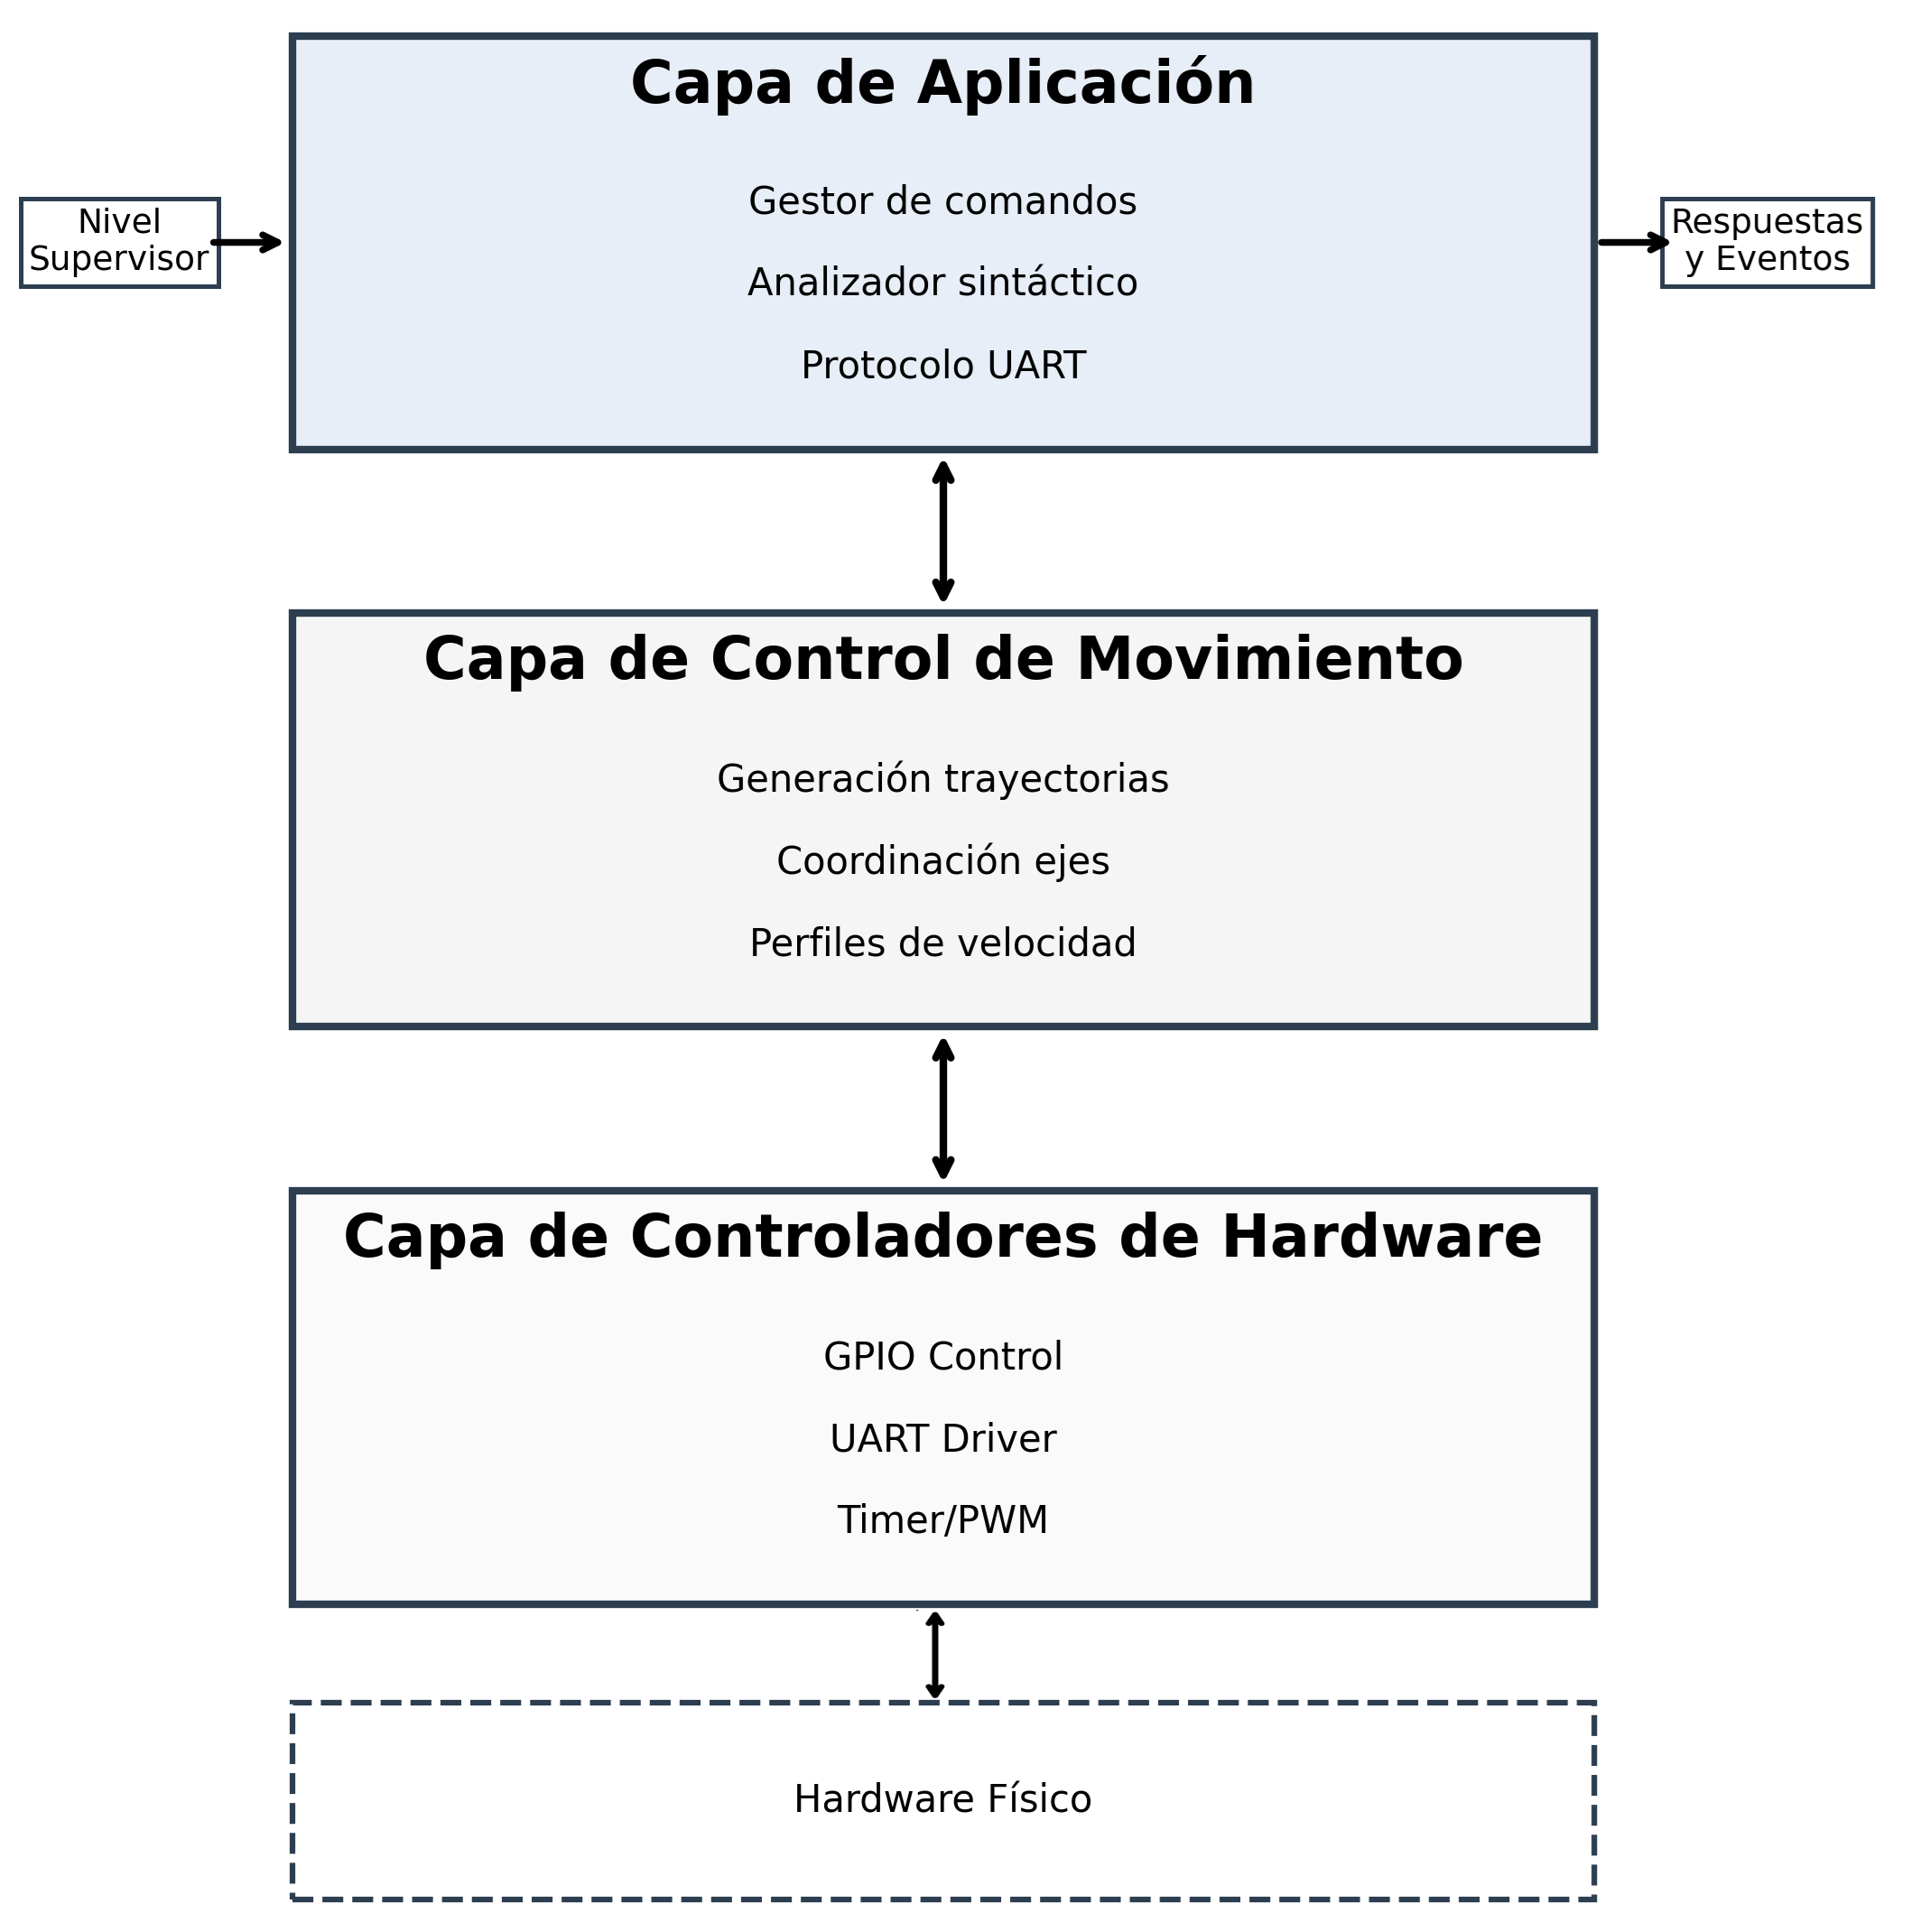
\includegraphics[width=0.85\textwidth]{imagenes/arquitectura_regulatorio_capas.png}
    \caption{Arquitectura en capas del firmware del Nivel Regulatorio}
    \label{fig:arquitectura_regulatorio}
\end{figure}

\subsubsection{Loop Principal y Modelo de Ejecución}

El firmware opera con un modelo híbrido interrupt-driven + polling:

\textbf{Procesamiento por interrupciones}:
\begin{itemize}
    \item \textbf{UART RX}: Recepción de bytes en buffer circular (ISR: \texttt{USART0\_RX\_vect})
    \item \textbf{Timer1}: Generación de pulsos de steppers a frecuencia variable (ISR: \texttt{TIMER1\_COMPA\_vect})
    \item \textbf{Timer4/5}: Generación de señales PWM para servos (hardware PWM, sin ISR)
\end{itemize}

\textbf{Loop principal}: Ejecuta continuamente a frecuencia aproximada de 10 kHz, realizando tres tareas principales:
\begin{itemize}
    \item Actualización de perfiles de velocidad para motores paso a paso
    \item Verificación y actualización de trayectorias de servomotores
    \item Gestión del estado del gripper y sus transiciones
\end{itemize}

Este diseño garantiza que la generación de pulsos de steppers (crítica en tiempo) se maneja en interrupciones con latencia <10µs, mientras que tareas menos críticas se ejecutan en el loop principal con latencia <100µs.

\subsubsection{Gestión de Estado Global}

El firmware mantiene estado distribuido en estructuras estáticas:

\begin{itemize}
    \item \texttt{stepper\_state}: Posición actual (en pasos), velocidad actual, aceleración, dirección para cada eje
    \item \texttt{servo\_positions}: Ángulos actuales de servos 1 y 2
    \item \texttt{gripper\_state}: Estado (abierto/cerrado), posición en pasos, flag de movimiento activo
    \item \texttt{limits\_status}: Bits de estado de 4 finales de carrera
\end{itemize}

El acceso concurrente se gestiona mediante:
\begin{itemize}
    \item Variables volátiles para datos compartidos entre ISR y loop principal
    \item Secciones críticas con \texttt{cli()}/\texttt{sei()} para operaciones atómicas
    \item Flags de sincronización para eventos asíncronos
\end{itemize}

\subsubsection{Determinismo Temporal}

El firmware garantiza determinismo mediante:

\textbf{Frecuencia fija de Timer1}: Configurado con TOP variable que se recalcula cada ciclo basado en el perfil de velocidad actual. Esto permite ajustar dinámicamente la frecuencia de pulsos manteniendo el ciclo de interrupción predecible.

\textbf{Ejecución acotada del loop}: Cada iteración del loop principal toma <100µs (medido), permitiendo rate de actualización >10kHz suficiente para mantener perfiles de velocidad suaves.

\textbf{Prioridades de interrupción}: Timer1 (steppers) tiene máxima prioridad, UART menor prioridad. Si llega un byte UART durante generación de pulso stepper, se bufferea y procesa después sin pérdida.

Esta arquitectura permite que el nivel regulatorio ejecute movimientos coordinados con precisión submilimétrica (<0.1mm de error acumulado en trayectorias de 500mm) mientras mantiene comunicación bidireccional fluida con el supervisor.
